\documentclass{article}

%\usepackage[backend=biber]{biblatex}
\usepackage{enumitem}
\usepackage[final]{graphicx}           % Extended \includegraphics         
\usepackage[reqno]{amsmath}            % Higher mathematics
\usepackage{hyperref}           
\usepackage[margin = 0.5in]{geometry}
\usepackage{float}
\usepackage{amssymb}            % special math fonts
\usepackage{amsmath}
\usepackage{siunitx}
\usepackage{enumitem}
\usepackage{cancel}
\usepackage{braket}
\usepackage{tikz}
\usepackage{physics}
\usepackage{subcaption}
\usepackage{lineno}
\usepackage{bbm}%% make sure you have the nature.cls and naturemag.bst files where
%% LaTeX can find them
%\bibliographystyle{naturemag}
\linenumbers

\title{The search for missing matter using the Universe's baby pictures}

%% Notice placement of commas and superscripts and use of &
%% in the author list

\author{Word Count = 1007}


\begin{document}

\maketitle

% \begin{affiliations}
Mitchell de Zylva, Astronomer, The University of Melbourne, Victoria, Australia
% \end{affiliations}

%\begin{abstract}


\begin{figure}[H]
    \label{fig:planck}
    \begin{center}
        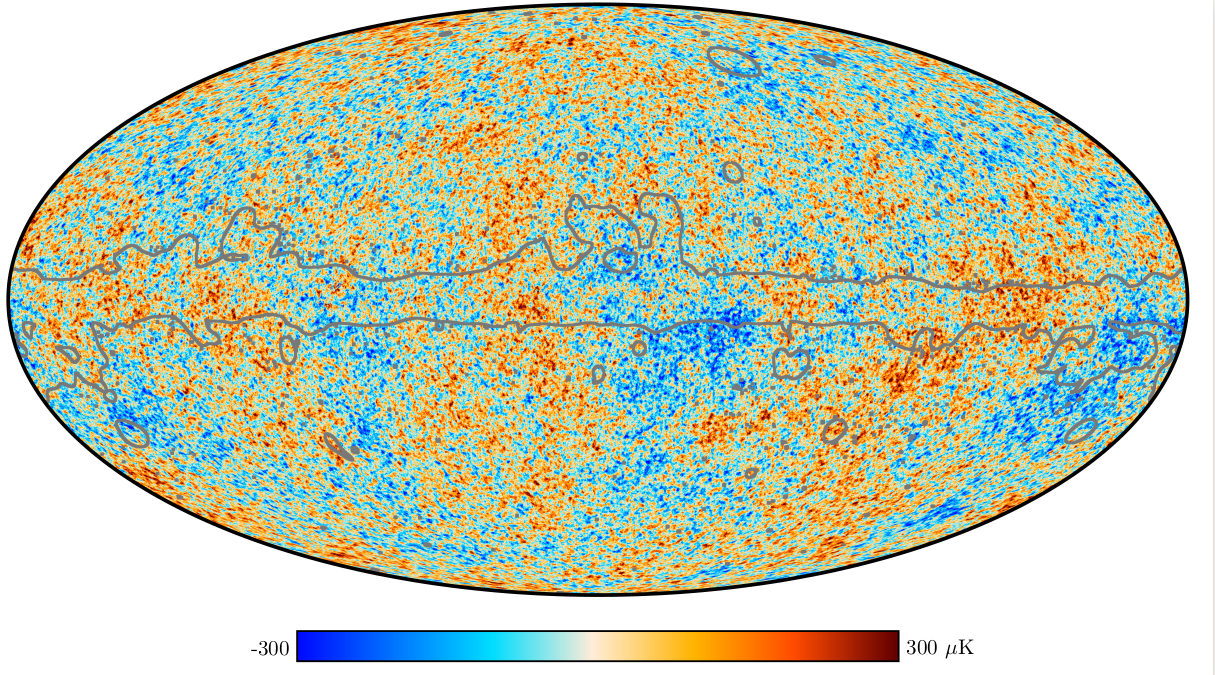
\includegraphics[scale=0.3]{planck_cmb.png}
        \caption{The Cosmic Microwave Background from the \textit{Planck} Satellite (Grey lines indicate the location of the Milky Way Galaxy)}
    \end{center}
\end{figure}

\section{The Cosmic Microwave Background}

Fifty five years after its accidental discovery, the first image of a baby universe has still not given up all its secrets. The afterglow of the Big Bang, known as the Cosmic Microwave Background (CMB), is the only faint remnant of the young universe currently still visible in the sky, and has been central in ushering in a golden age of cosmology. This golden age has been instrumental in defining many of the models used to describe the universe, but if even a single one of these is wrong, the whole thing may collapse like a house of cards. 

The CMB, the before picture to the breathtaking after pictures seen through the Hubble Space Telescope, is made up of microwaves which carry very low power, and the characteristic splotches in it provide key insights into conditions in the early universe. This allows astronomers to determine characteristics, such as the relative proportions of matter, dark matter, dark energy, and other fundamental parameters. These splotches yield the most precise measures of the age, geometry, and composition of the universe to date. 

In more recent years, a number of experiments have been done specifically to examine the properties of the CMB, including the Atacama Cosmology Telescope in Chile, the South Pole Telescope, and the European Space Agency's \textit{Planck} Satellite. These experiments have broadened the scope of the original detection, leading to the collection of an unprecedented amount of data, and its application across numerous areas of astronomy. 

\section{The Missing Baryon Problem}
The CMB has allowed scientists to determine with a very high level of confidence the composition of the universe. The universe is broadly comprised of light, regular matter, and the infamous dark matter and dark energy, the precise ratios of which are very tightly constrained. 

However when astronomers look at the sky, and measure the amount of matter they see with telescopes, it becomes apparent that only about half of the universe's regular matter - known collectively as 'baryons' - is present in the light emitted from stars and galaxies. This begs two very important questions, what if our models are wrong, and if not, where is all the missing matter? 

It is clear that the matter must be there, since it is very easy to discern between dark matter and baryons in physical models. The universe could not have evolved to be what we see today if that fraction wasn't correct. But it was also apparent that only about 10 percent of baryons exist in galaxies themselves, with some 30 to 40 percent existing in gas clouds surrounding galaxies. This still leaves a large fraction unaccounted for. 

One possible answer arises from simulations. Astronomers can model the evolution of the universe by tracking individual clumps of gas, and when they evolve them forward in time, they notice something interesting. The gas that doesn’t collapse to form galaxies stretches out into long filaments.
\begin{figure}[H]
    \begin{center}
        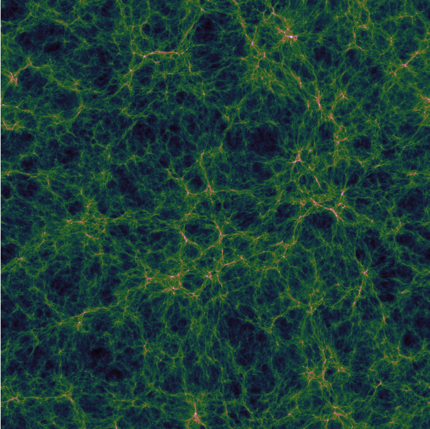
\includegraphics[scale=0.4]{tiamat-1.png}
        \caption{The Large-Scale Structure of the Universe, from the \textit{dragons} Simulations }
    \end{center}
\end{figure}

These filaments contain very small amounts of matter, superheated to temperatures between thousands and millions of degrees, and spread out over the vast reaches of space. The combination of their high temperature and these distances makes these filaments very sparse - only a few atoms per cubic meter. 

Detecting these filaments has proven to be a difficult task, since the scarcity of the gas makes it very unlikely that there will be any observable signal. The only possible method of direct detection of this matter involves using a quasar, a galaxy with a very active super-massive black hole at its centre, as a backlight. Unfortunately this is an incredibly rare event, since it requires us to not only find such an object, but to also capture it with a telescope while its beam is aligned with the Earth. 

\section{A new use for the oldest light in the universe}

One possible solution is to use the CMB itself. At a fundamental level, the CMB is just light, sitting at the edge of the observable universe, and light is interactive. It is distorted by the matter between it and our detectors in a number of different ways.

Scientists appeal first to the phenomenon of Compton Scattering, which was subject of the 1927 Nobel Prize, and named after its discoverer, Arthur Holly Compton. This effect describes how light can exchange some of its energy with electrons, and vice versa. Since there is hot gas in between us and the CMB, there will be sections of the sky which will have absorbed some energy from the intervening gas, and look brighter than its surroundings. 

On their own, the signals obtained by this technique is too small for us to detect for a single filament; there is just not enough matter. We can however, use this fact to our advantage, since by definition, the noise in the signal is random. If we add multiple detections together, the signal gets stronger as the random noise gets weaker. Therefore, we can make a direct detection if we add multiple images on top of each other.

\section{Tracing the Large-Scale Structure of the Universe}

With this in mind, scientists know that they must use locations where they expect to find the missing matter in order to make a detection of any kind. To do so, they look to comprehensive galaxy surveys, such as the Sloan Digital Sky Survey (SDSS) and the Dark Energy Survey (DES), which have created some of the most detailed three-dimensional maps of the universe we have to date.

Once the galaxies are located, they are paired up based on whether they are likely to have a filament connecting them, and located in the CMB. The signals are then added together, hopefully revealing the missing baryons.

This search has been shown to work with low resolution images of the CMB, revealing the missing matter with relative certainty, however there is still more to be done to confirm this. By accessing higher resolution images, scientists hope to confirm the location of the missing baryon fraction, to remove any shred of doubt as to the validity of current cosmological models.
% Citation of Einstein's paper \cite{Einstein}.

%\bibliographystyle{naturemag}
%\bibliography{sample}
\end{document}
% Citation of Einstein's paper \cite{Einstein}.
